\lyxframe{Iterative Algorithms}
\begin{columns}
\begin{column}{0.4\textwidth}
\only<1>{
\centering
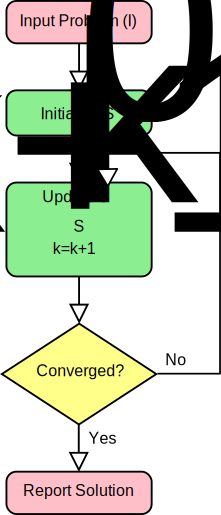
\includegraphics[height=0.8\textheight]{images/iterative-algm}

}

\end{column}
\begin{column}{0.6\textwidth}
\begin{block}{Iterative Algorithms}
\begin{itemize}
\item A typical iterative algorithm has following components:
\begin{enumerate}
\item The input problem;
\item Intermediate variable; 
\item Update relation; 
\item Convergence checking; and 
\item Solution. 
\end{enumerate}
\end{itemize}
\end{block}
\end{column}

\end{columns}

\lyxframeend{}

%%%%%%%%%%%%%%%%%%%%%%%%%%%%%%%%%%%%%%%%%%%%%%%%%%%%%%%%%
\lyxframe{Iterative Algorithm as State Machine}
\begin{columns}
\begin{column}{0.4\textwidth}
\only<1>{
\centering
\includegraphics[height=0.8\textheight]{images/iterative-sm/iterative-sm-1}

}
\only<2>{
\centering
\includegraphics[height=0.8\textheight]{images/iterative-sm/iterative-sm-2}

}
\only<3>{
\centering
\includegraphics[height=0.8\textheight]{images/iterative-sm/iterative-sm-3}

}
\only<4>{
\centering
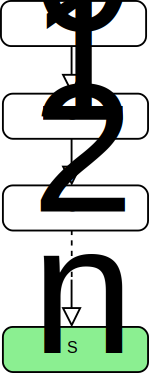
\includegraphics[height=0.8\textheight]{images/iterative-sm/iterative-sm-4}

}


\end{column}
\begin{column}{0.6\textwidth}
\begin{block}{Iterative Algorithms as State Machines}
\begin{itemize}
\item An iterative algorithm can be viewed as state machine.
\item State of the algorithm: subset of intermediate variables required for continued execution of the algorithm.
\item Starts with an initial state $S_{0}$
\item Uses update relation to transition from one state to another 
\[
S_{k+1} \leftarrow S_{k}
\]
\end{itemize}
\end{block}
\end{column}
\end{columns}

\lyxframeend{}

%%%%%%%%%%%%%%%%%%%%%%%%%%%%%%%%%%%%%%%%%%%%%%%%%%%%%%%%%
\lyxframe{Single Fault in Iterative Algorithm}
\begin{columns}
\begin{column}{0.5\textwidth}
\only<1>{
\centering
\includegraphics[height=0.6\textheight]{images/iterative-fault}

}
\only<2>{
\centering
\includegraphics[height=0.6\textheight]{images/iterative-valid}

}
\only<3>{
\centering
\includegraphics[height=0.6\textheight]{images/iterative-invalid}

}
\end{column}
\begin{column}{0.5\textwidth}
\begin{block}{Valid and Invalid States}

\begin{itemize}
\item Valid state: under fault-free execution of the algorithm from that state, the algorithm will converge to the correct solution; otherwise invalid. 
\item In fault free execution, the algorithm always remains in a valid state.
\item Any hardware fault can cause the algorithm to reach an invalid state.
\item In general determining whether a given state is valid or not, is non-trivial.     
\end{itemize}
\end{block}
\end{column}
\end{columns}


\lyxframeend{}

%%%%%%%%%%%%%%%%%%%%%%%%%%%%%%%%%%%%%%%%%%%%%%%%%%%%%%%%%
\lyxframe{Self-stabilizing Algorithms}
\begin{columns}
\begin{column}{0.5\textwidth}
\only<1>{
\centering
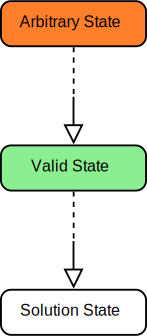
\includegraphics[height=0.6\textheight]{images/self-stab}

}

\end{column}
\begin{column}{0.5\textwidth}
\begin{block}{Self-stabilizing Algorithms}
\begin{itemize}
\item Starting from any arbitrary state, valid or invalid, a self-stabilizing algorithm will reach a valid in finite number of steps. 
\item Natural fault-tolerance mechanism.
\item Examples: Stationary iterations, Newton Iteration. 
\item Self-stabilization is a \emph{strong} property.
%, as it does not assume any thing about history of computation.
\end{itemize}
\end{block}

\begin{block}{Scala'13}
\begin{itemize}
\item Self-stabilizing Steepest Descent and Conjugate Gradient.
\item Periodic state correction.
\item May not be generalized to all iterative algorithms.
\end{itemize}
\end{block}
\end{column}
\end{columns}

\lyxframeend{}

%%%%%%%%%%%%%%%%%%%%%%%%%%%%%%%%%%%%%%%%%%%%%%%%%%%%%%%%%
\lyxframe{Self-Correcting Algorithms}
\begin{columns}
\begin{column}{0.5\textwidth}
\only<1>{
\centering
\includegraphics[height=0.6\textheight]{images/self-correction}

}

\end{column}
\begin{column}{0.5\textwidth}
\begin{block}{Self-correcting Algorithms}
\begin{itemize}
\item A self-correcting algorithm is an iterative algorithm that, starting in some valid state, remains in a valid state or comes to a valid state in finite number of steps even if a fault occurs.
\item Requires that algorithm starts from a valid state. 
\item Uses information from previously known valid state.
% to detect invalid states, or to bring it to a valid state.
\item Example: Checkpoint-restart, FT-GMRES. 

\end{itemize}
\end{block}
\end{column}
\end{columns}


\lyxframeend{}

%%%%%%%%%%%%%%%%%%%%%%%%%%%%%%%%%%%%%%%%%%%%%%%%%%%%%%%%%
\lyxframe{Checkpoint-restart as a Self-correcting algorithm}
\begin{columns}
\begin{column}{0.5\textwidth}
\only<1>{
\centering
\includegraphics[height=0.6\textheight]{images/checkpt-restart}

}
\only<2>{
\centering
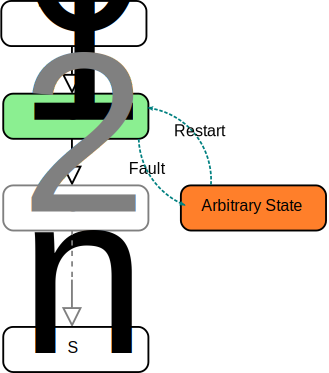
\includegraphics[height=0.6\textheight]{images/checkpt-restart-1}

}
\only<3>{
\centering
\includegraphics[height=0.6\textheight]{images/self-correction-1}

}

\end{column}
\begin{column}{0.5\textwidth}
\begin{block}{Checkpoint-restart based fault tolerance}
\begin{itemize}
\item<1-> Bring to valid state by restoring a check-pointed valid state.
\item<2-> \color{red} At high fault rate, algorithm will not make any progress.



\end{itemize}
\end{block}

\pause
\pause
{\color{dpg} Broader idea of self-correction is to use $S_{1}$ to construct an state 
\[\tilde{S}_{2} \approx S_{2}
\]
}
\end{column}
\end{columns}


\lyxframeend{}